\subsubsection{\large Diagrama de flujo \texttt{(interfaz.c)}}

% --- PROCEDIMIENTO 1 ---
\newpage
\paragraph{1. Procedimiento \texttt{interfaz\_grafica()}} ~\\
\begin{figure}[H]
    \centering
    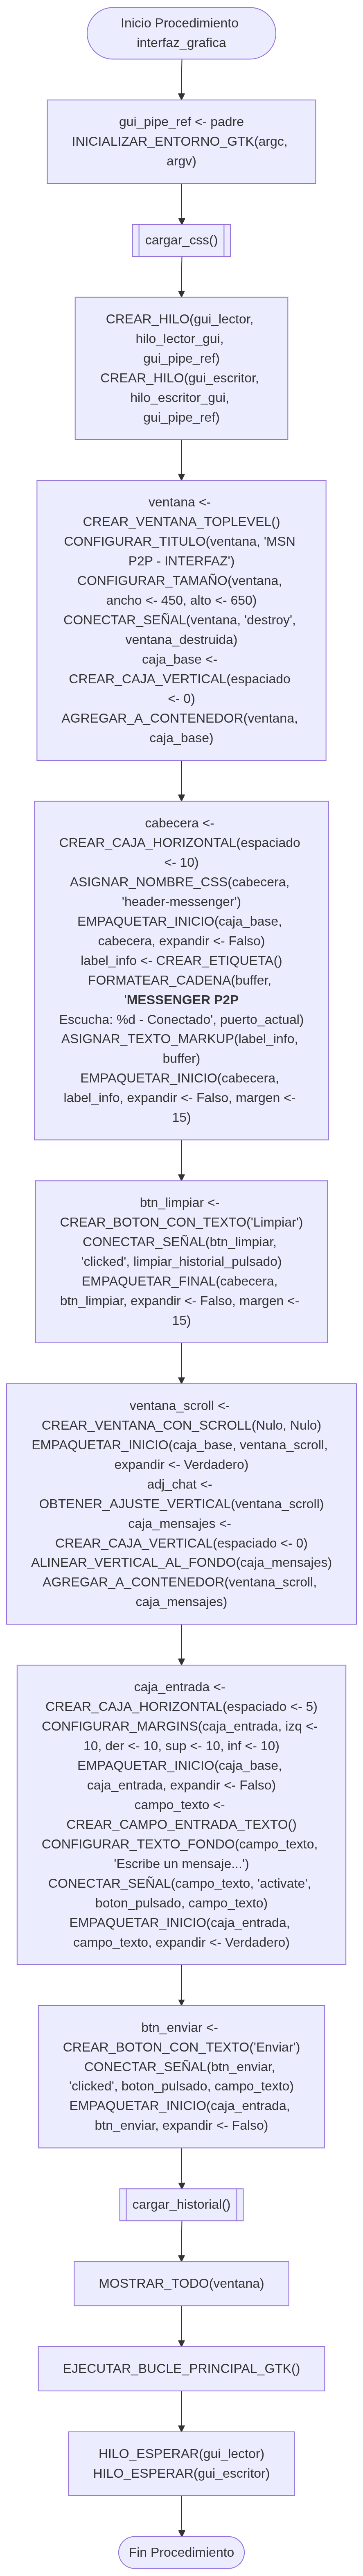
\includegraphics[width=0.15\textwidth]{Diagramas3/interfaz_grafica.png} 
\end{figure}

% --- FUNCION 2 ---
\newpage
\paragraph{2. Función \texttt{hilo\_lector\_gui()}} ~\\
\begin{figure}[H]
    \centering
    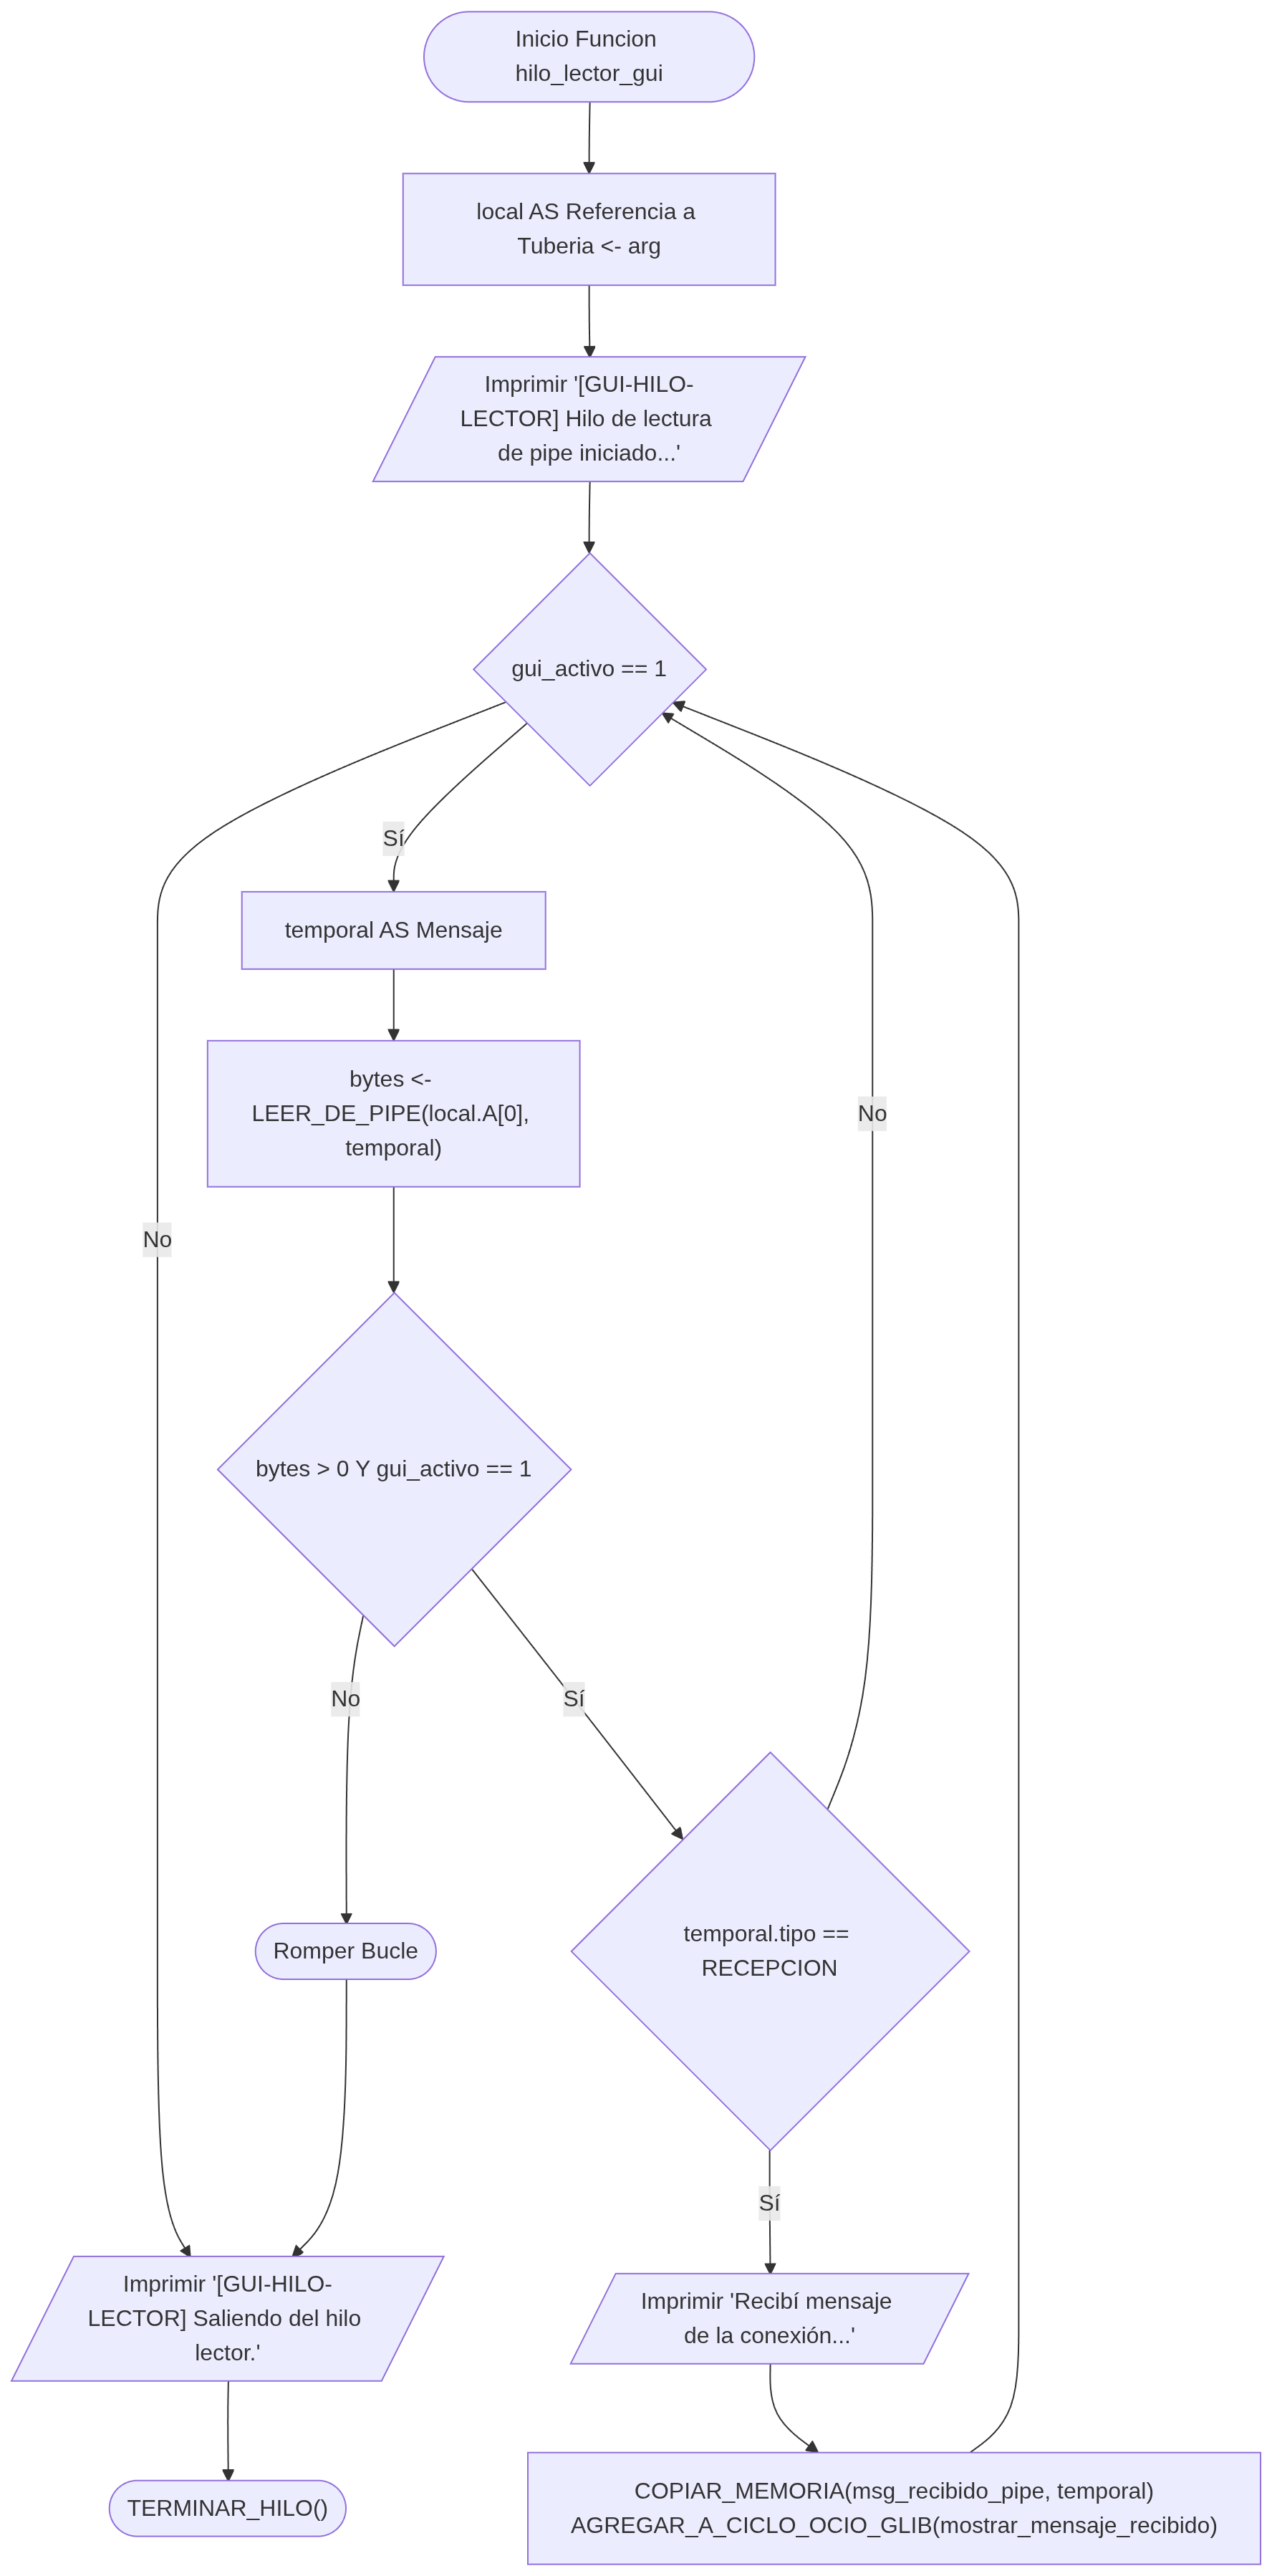
\includegraphics[width=0.5\textwidth]{Diagramas3/hilo_lector_gui.png} 
\end{figure}

% --- FUNCION 3 ---
\newpage
\paragraph{3. Función \texttt{hilo\_escritor\_gui()}} ~\\
\begin{figure}[H]
    \centering
    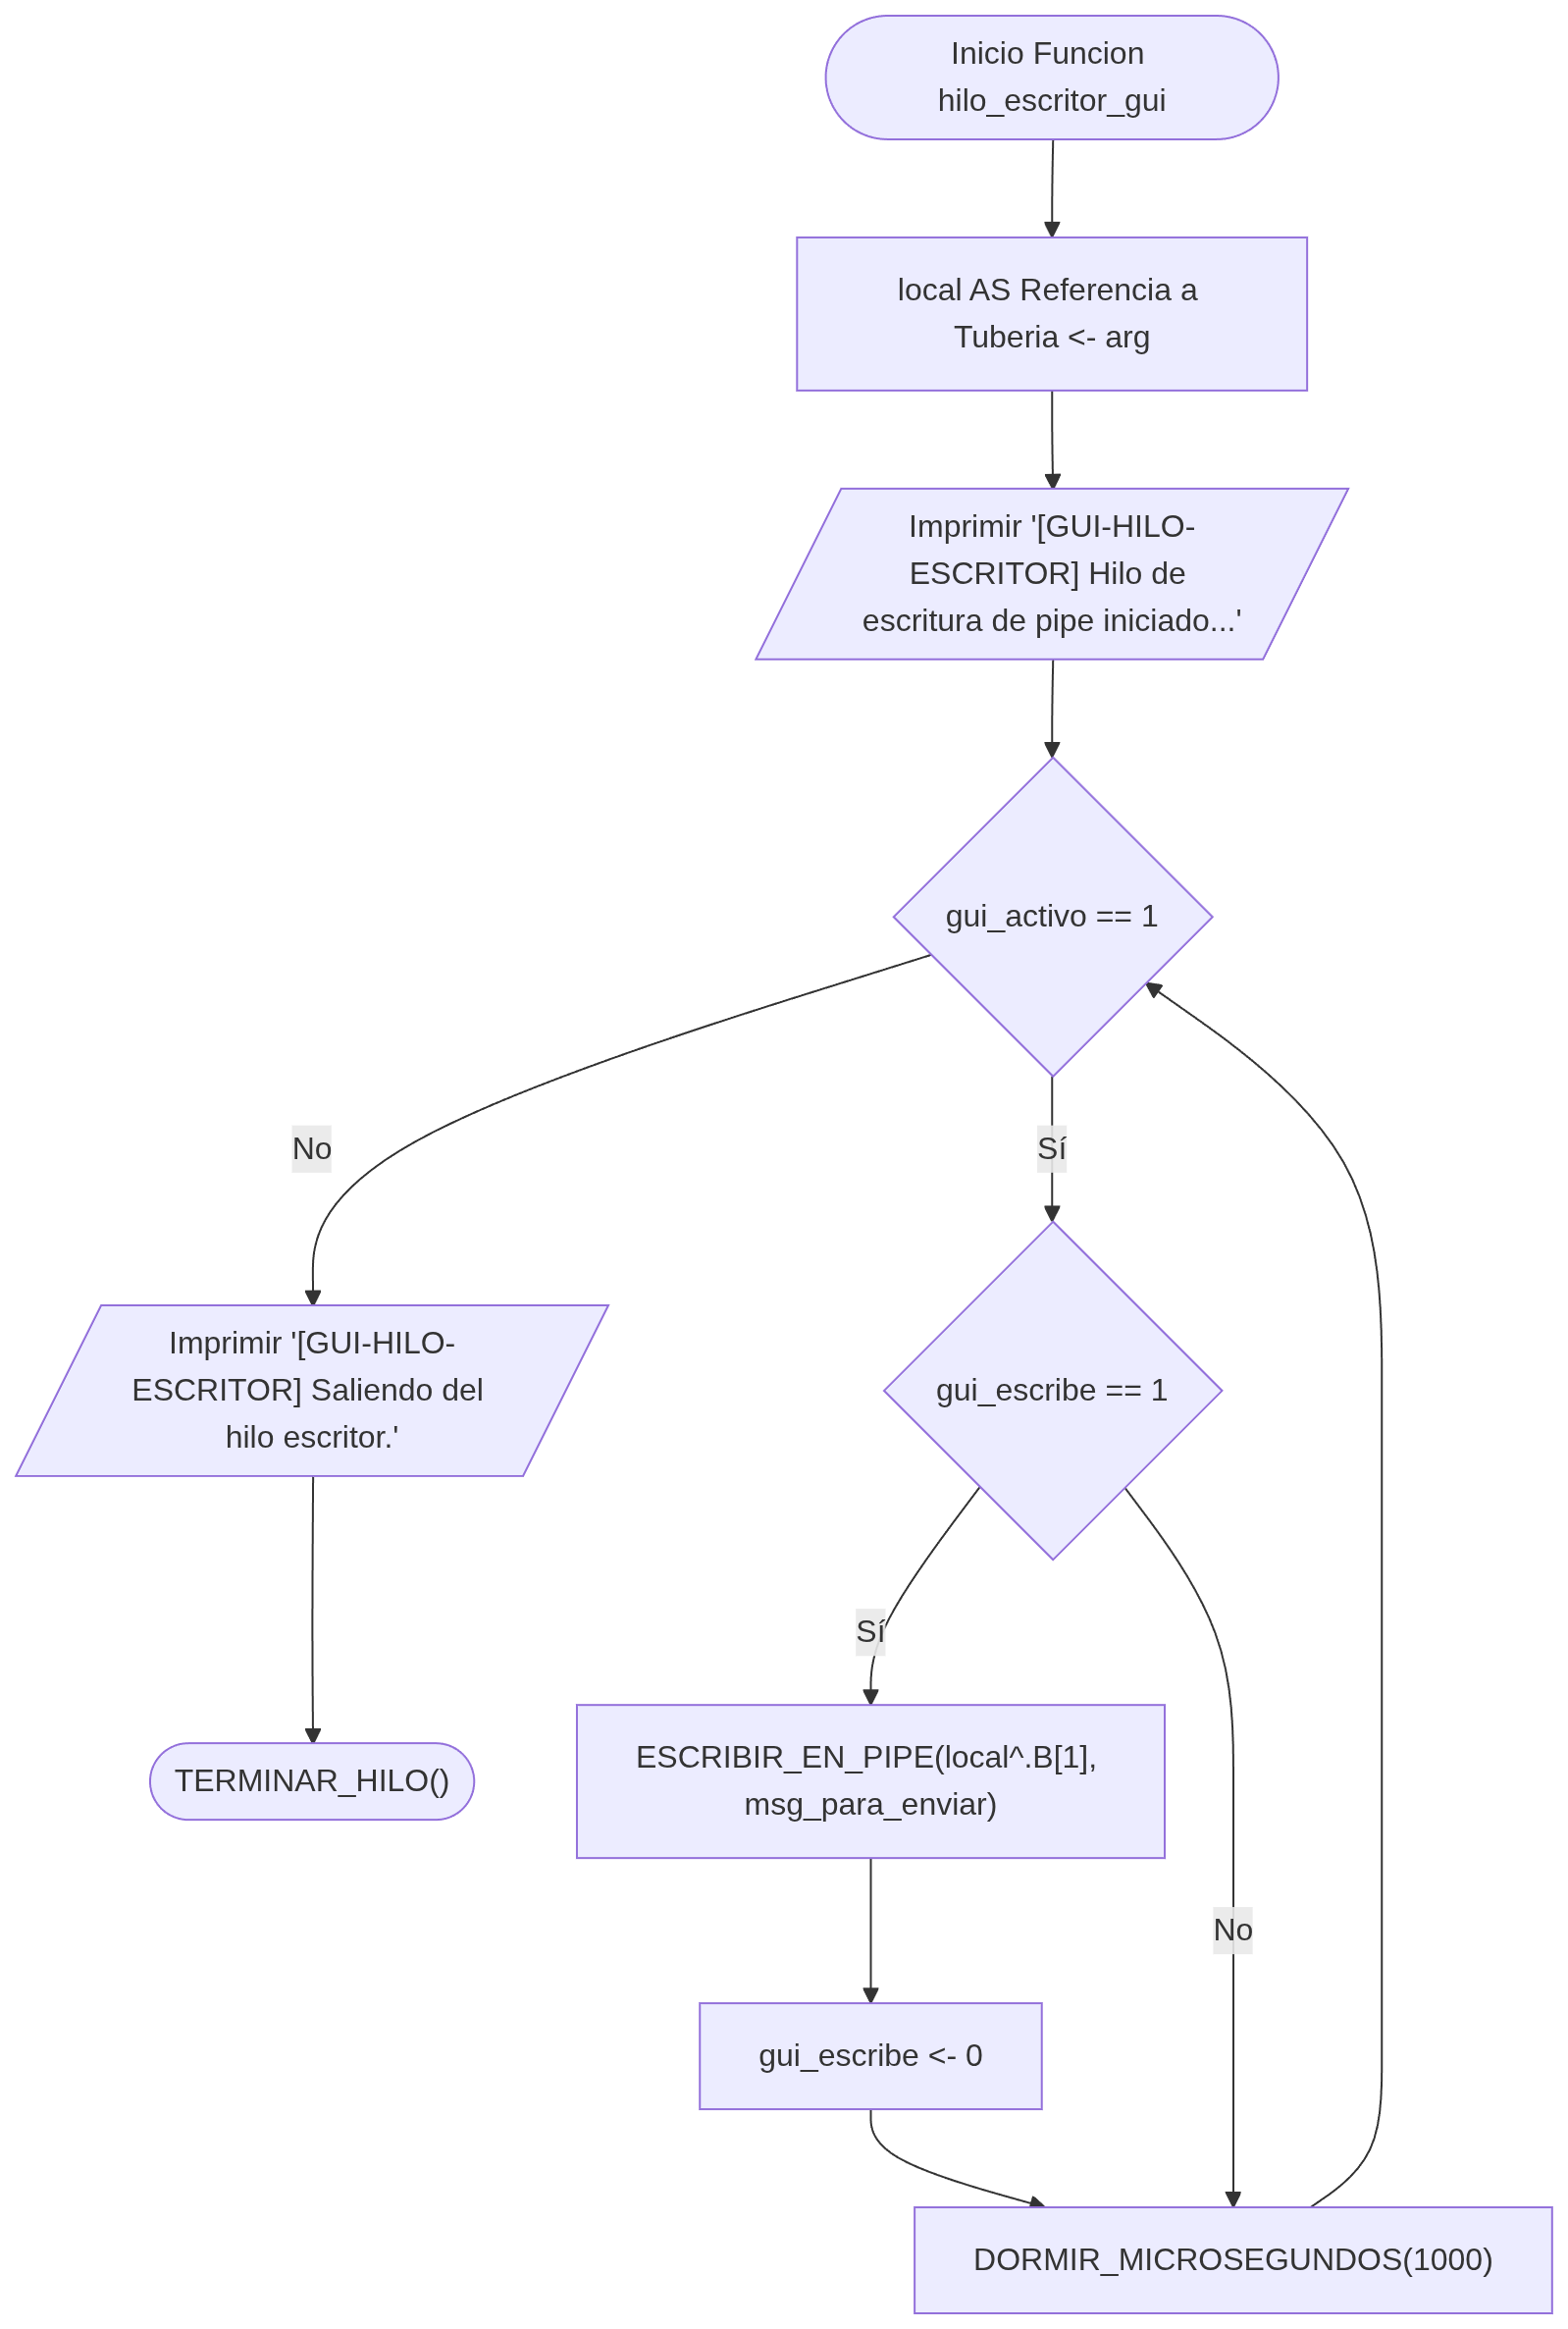
\includegraphics[width=0.5\textwidth]{Diagramas3/hilo_escritor_gui.png} 
\end{figure}

% --- PROCEDIMIENTO 4 ---
\newpage
\paragraph{4. Procedimiento \texttt{añadir\_burbuja()}} ~\\
\begin{figure}[H]
    \centering
    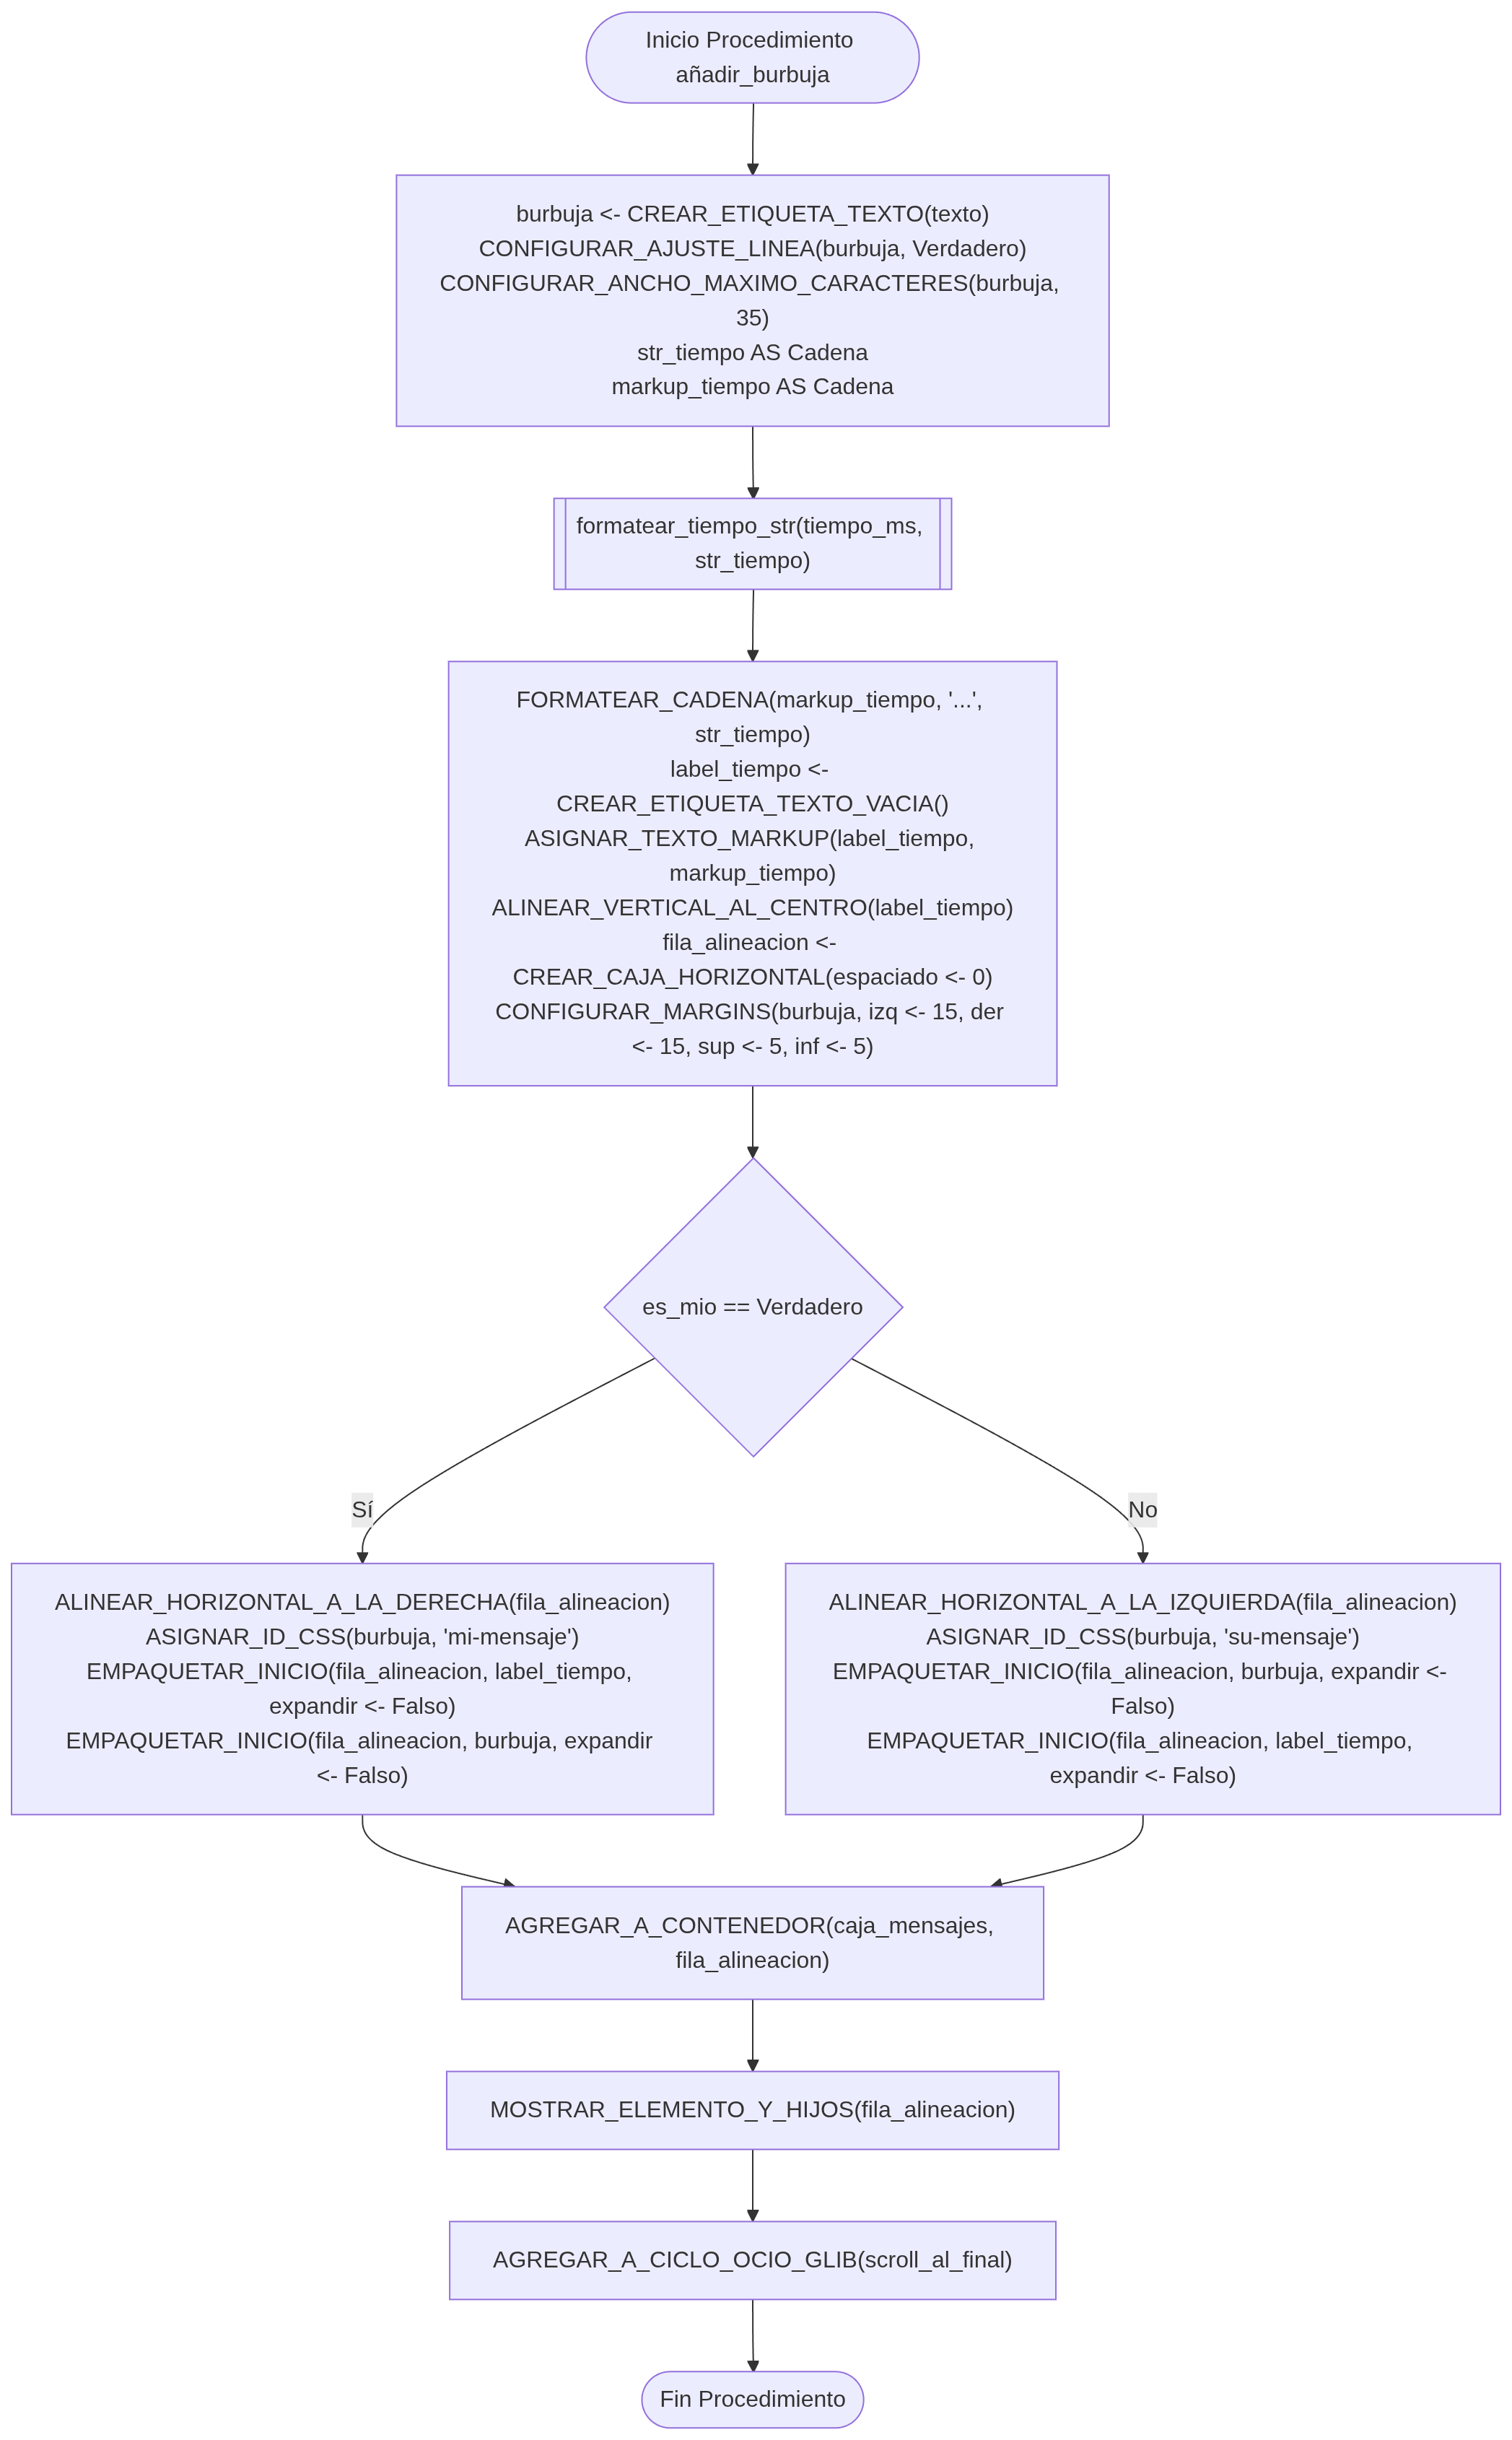
\includegraphics[width=0.6\textwidth]{Diagramas3/añadir_burbuja.png} 
\end{figure}

% --- PROCEDIMIENTO 5 ---
\newpage
\paragraph{5. Procedimiento \texttt{boton\_pulsado()}} ~\\
\begin{figure}[H]
    \centering
    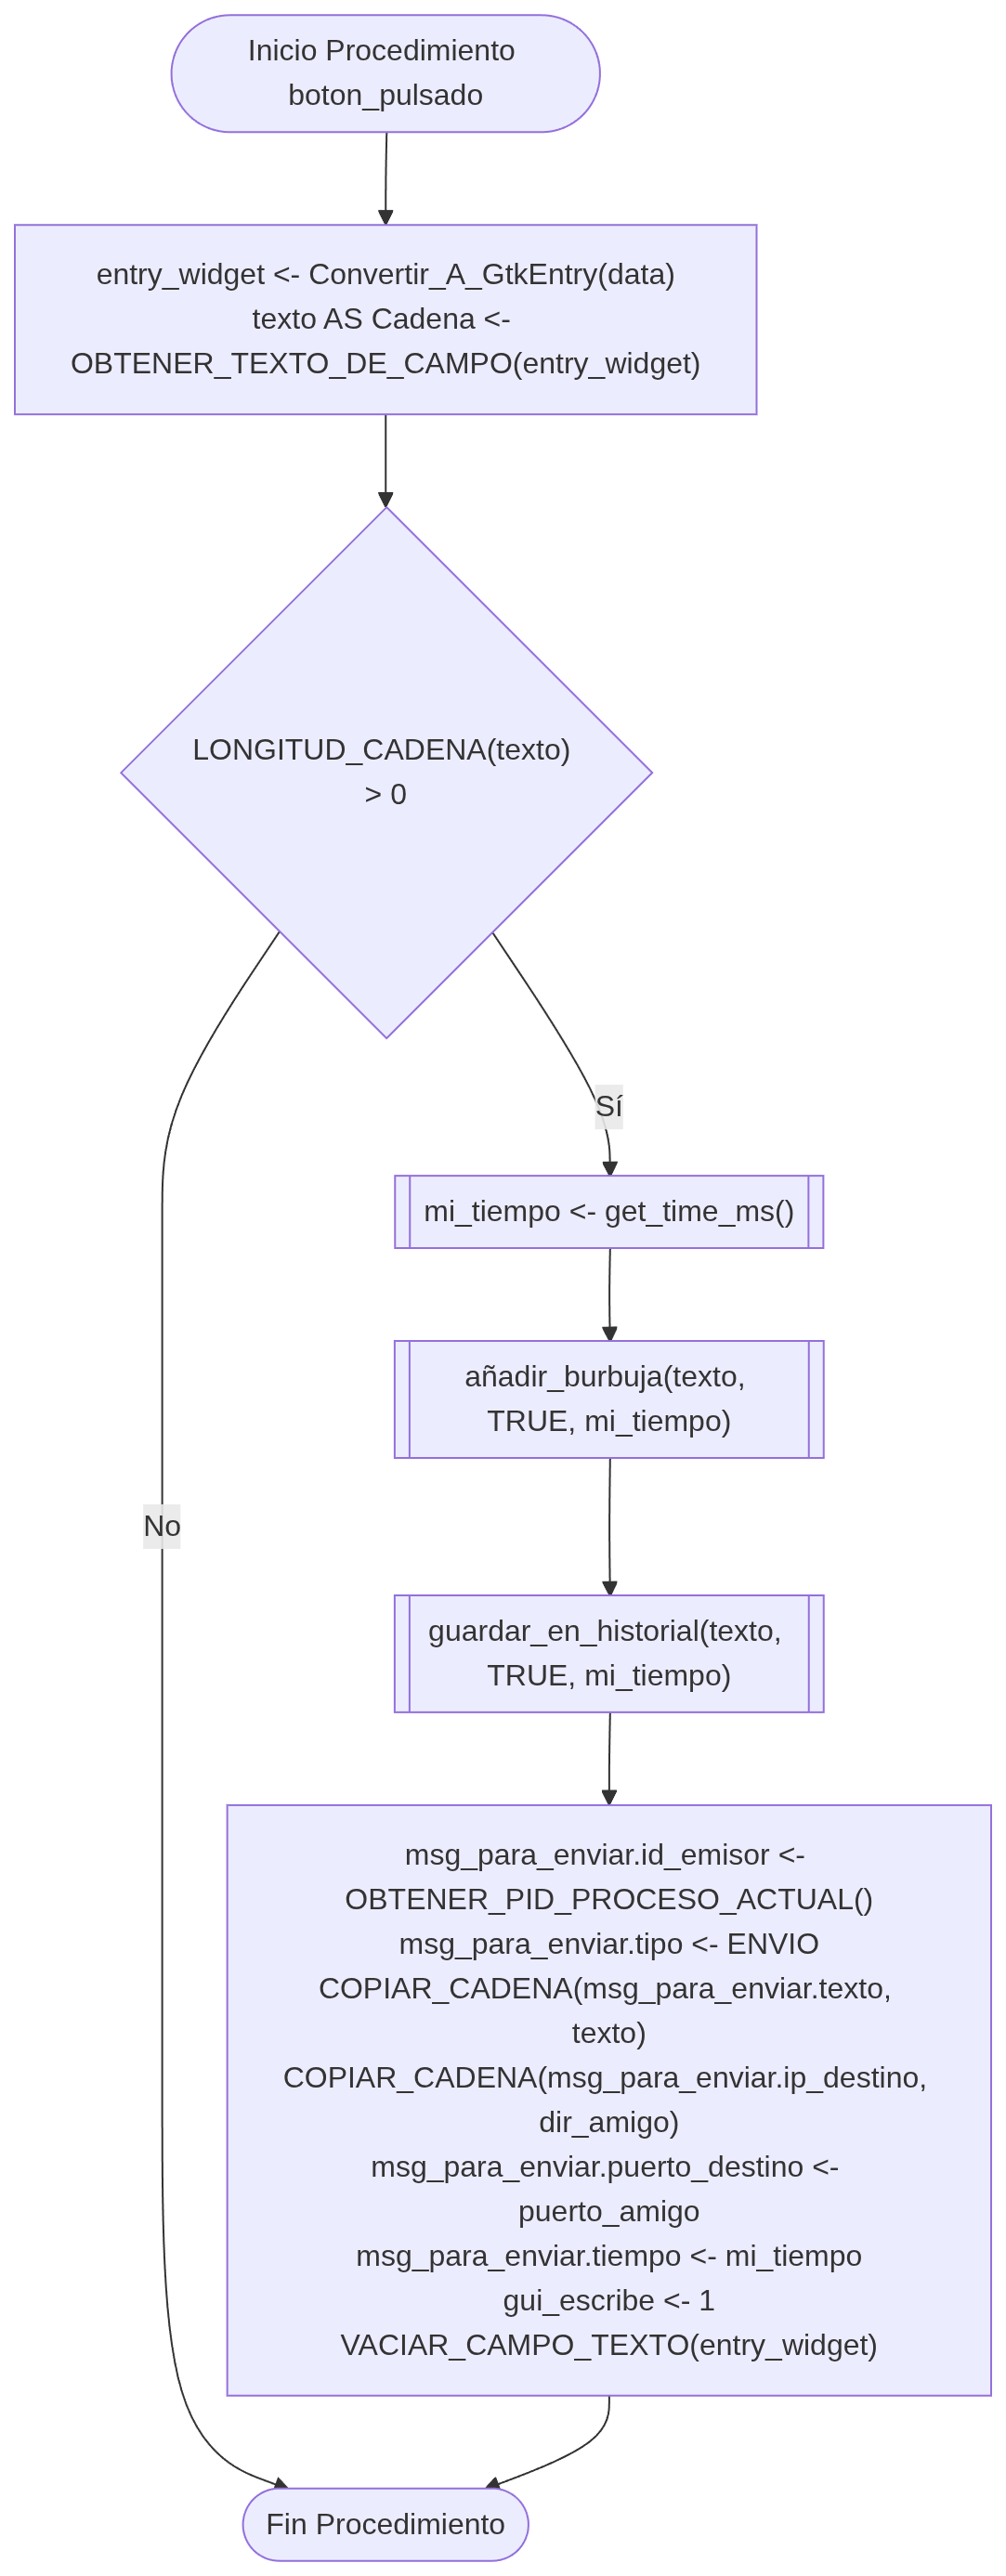
\includegraphics[width=0.4\textwidth]{Diagramas3/boton_pulsado.png} 
\end{figure}

% --- PROCEDIMIENTO 6 ---
\newpage
\paragraph{6. Procedimiento \texttt{ventana\_destruida()}} ~\\
\begin{figure}[H]
    \centering
    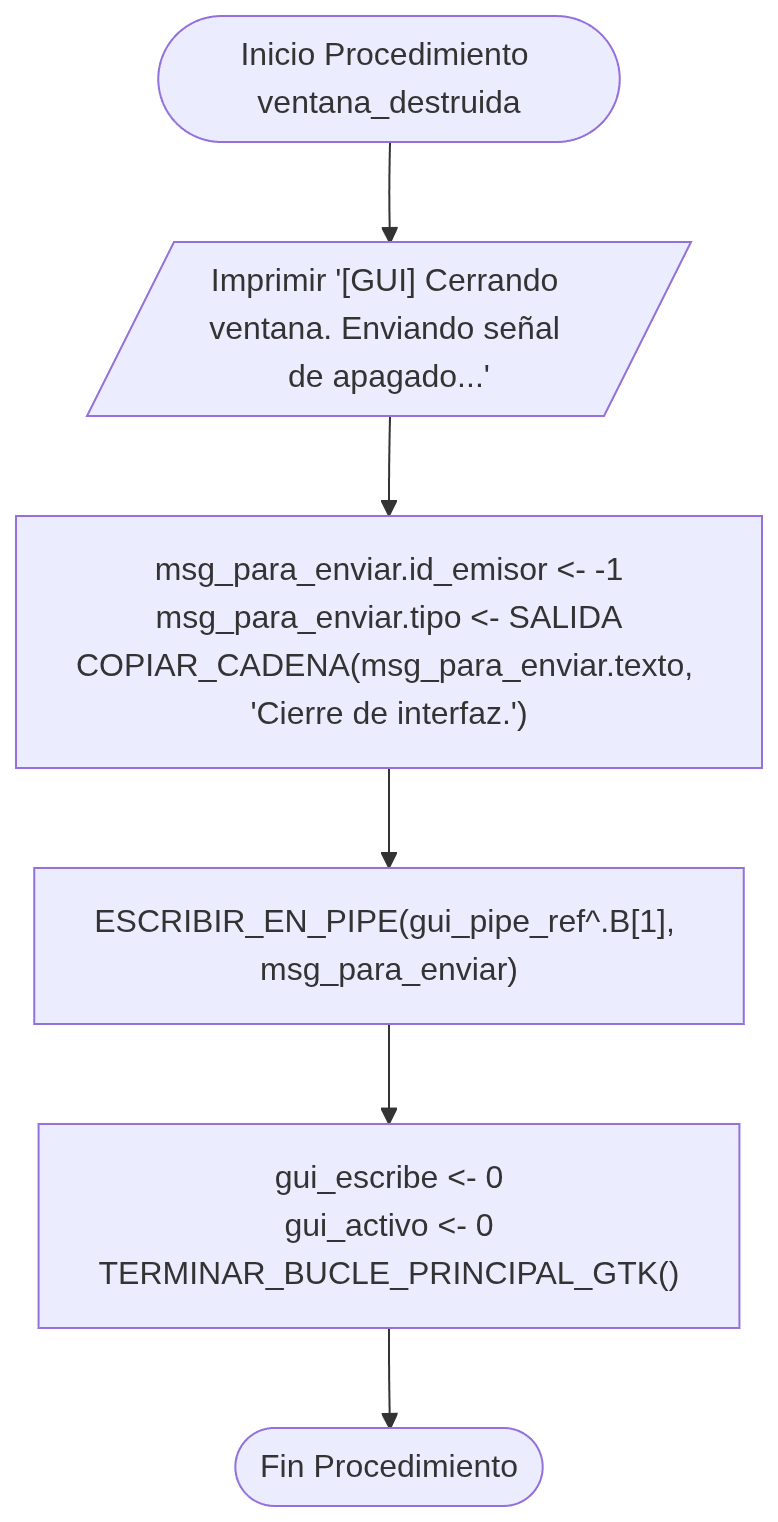
\includegraphics[width=0.4\textwidth]{Diagramas3/ventana_destruida.png} 
\end{figure}

% --- PROCEDIMIENTO 7 ---
\newpage
\paragraph{7. Procedimiento \texttt{guardar\_en\_historial()}} ~\\
\begin{figure}[H]
    \centering
    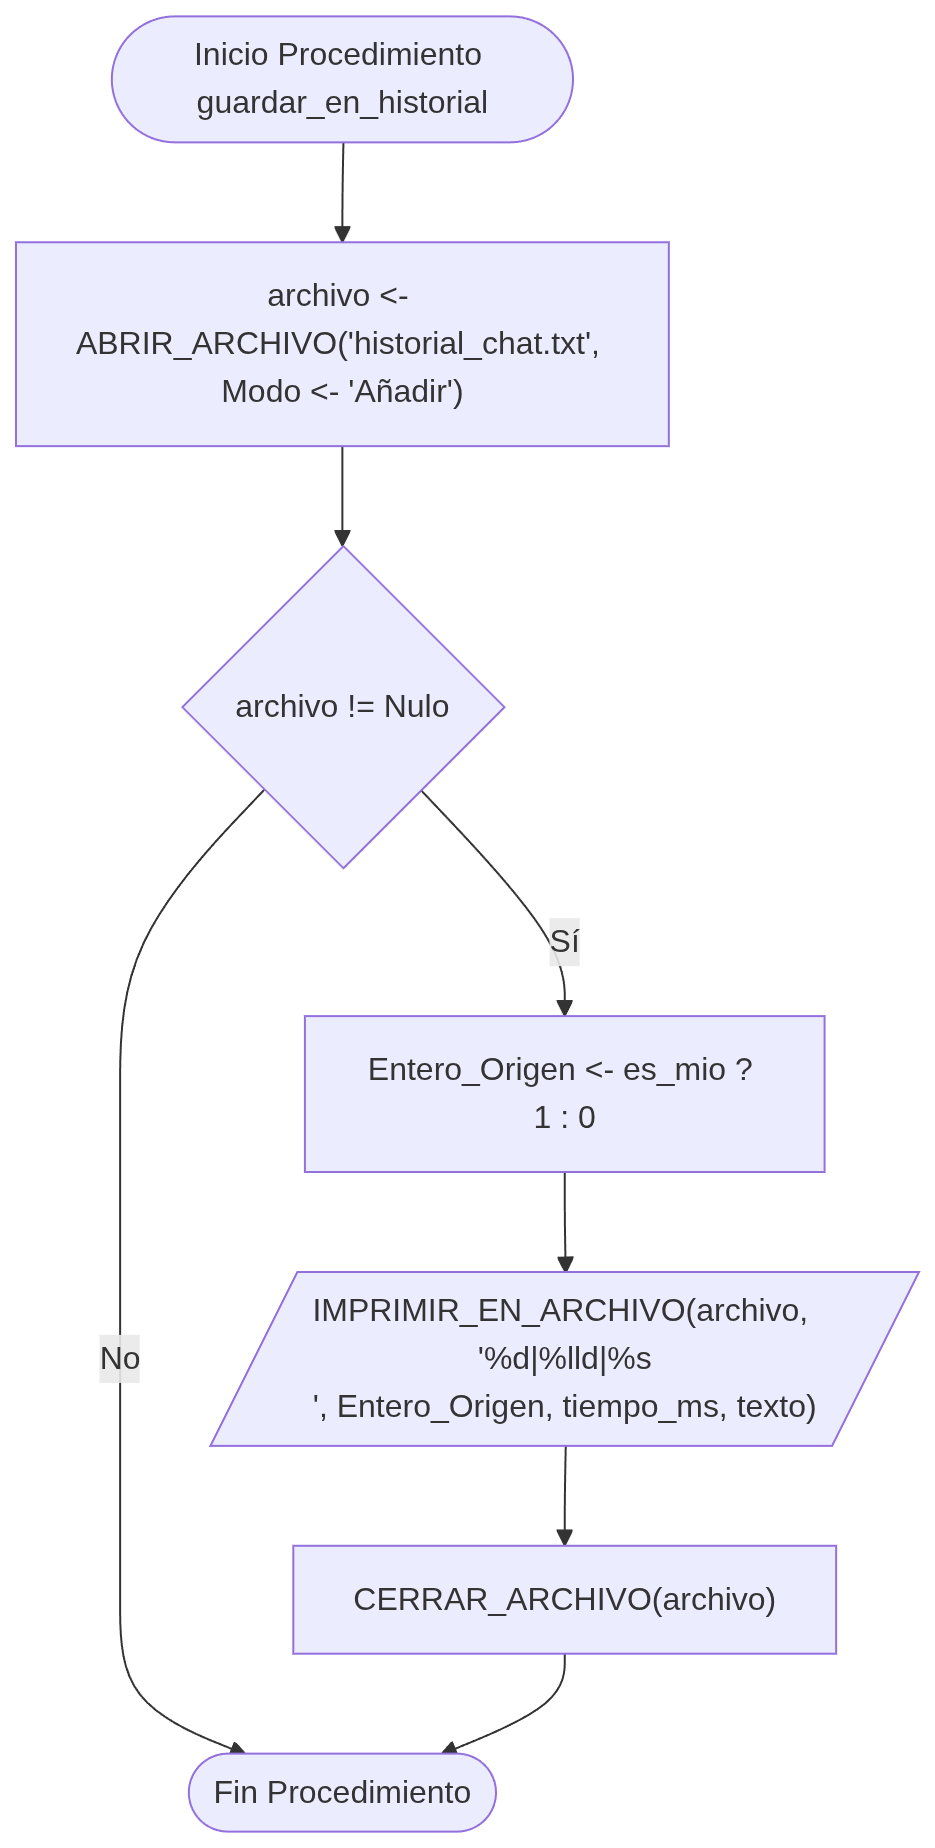
\includegraphics[width=0.4\textwidth]{Diagramas3/guardar_en_historial.png} 
\end{figure}

% --- PROCEDIMIENTO 8 ---
\newpage
\paragraph{8. Procedimiento \texttt{cargar\_historial()}} ~\\
\begin{figure}[H]
    \centering
    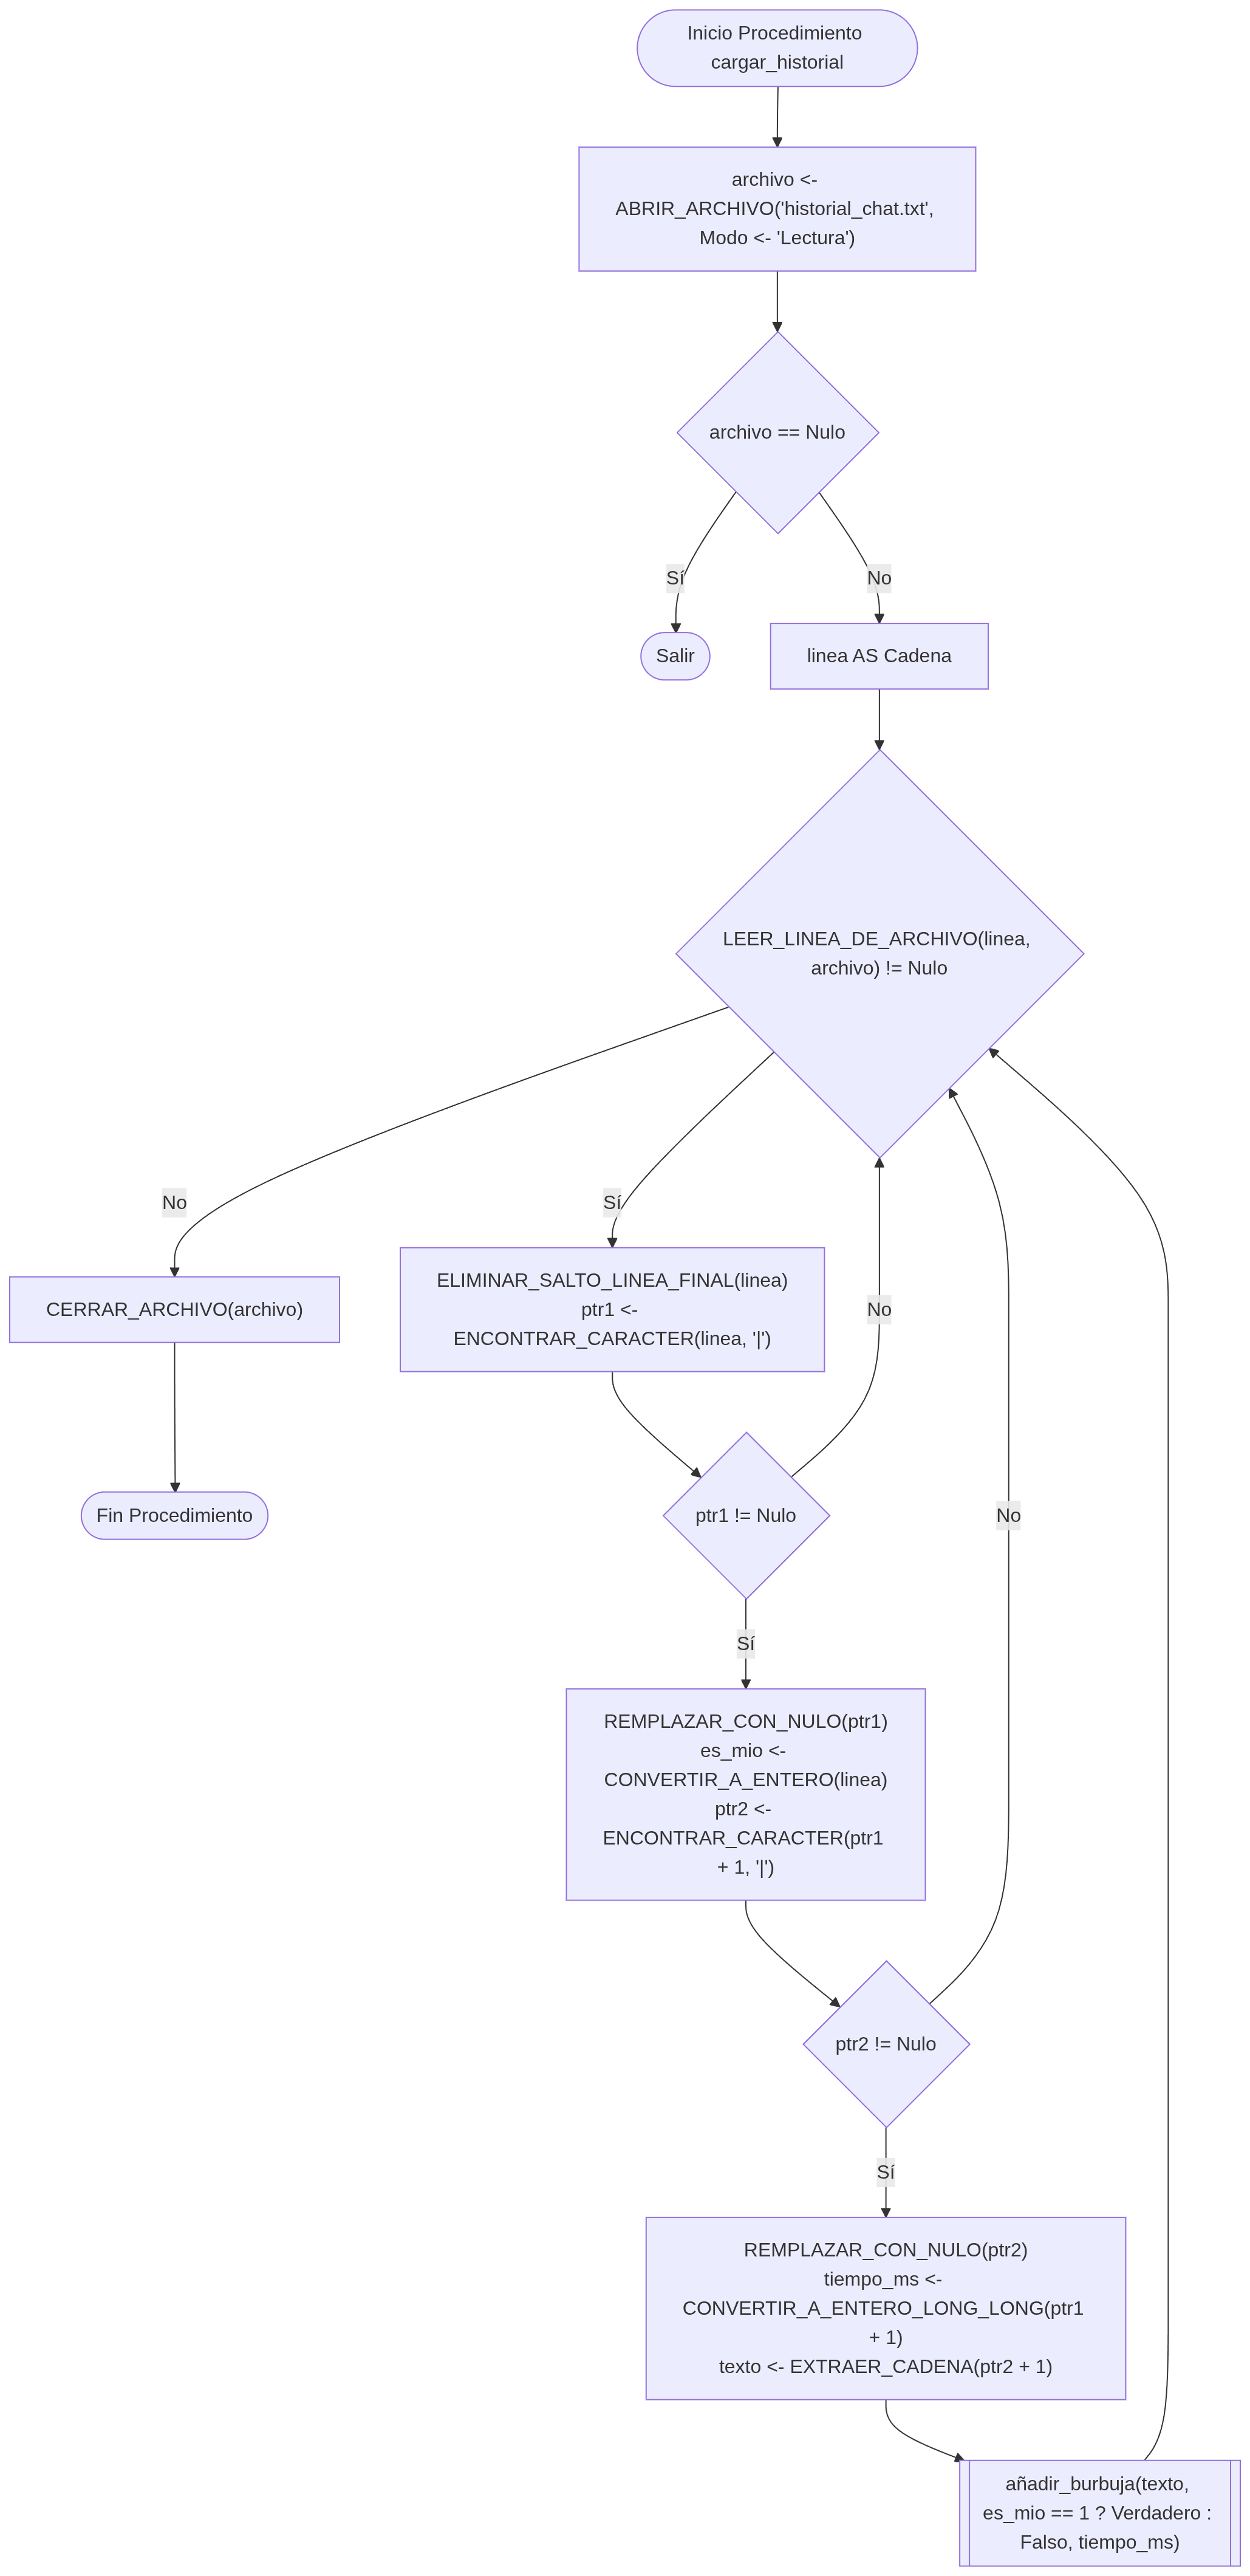
\includegraphics[width=0.5\textwidth]{Diagramas3/cargar_historial.png} 
\end{figure}

% --- PROCEDIMIENTO 9 ---
\newpage
\paragraph{9. Procedimiento \texttt{limpiar\_historial\_pulsado()}} ~\\
\begin{figure}[H]
    \centering
    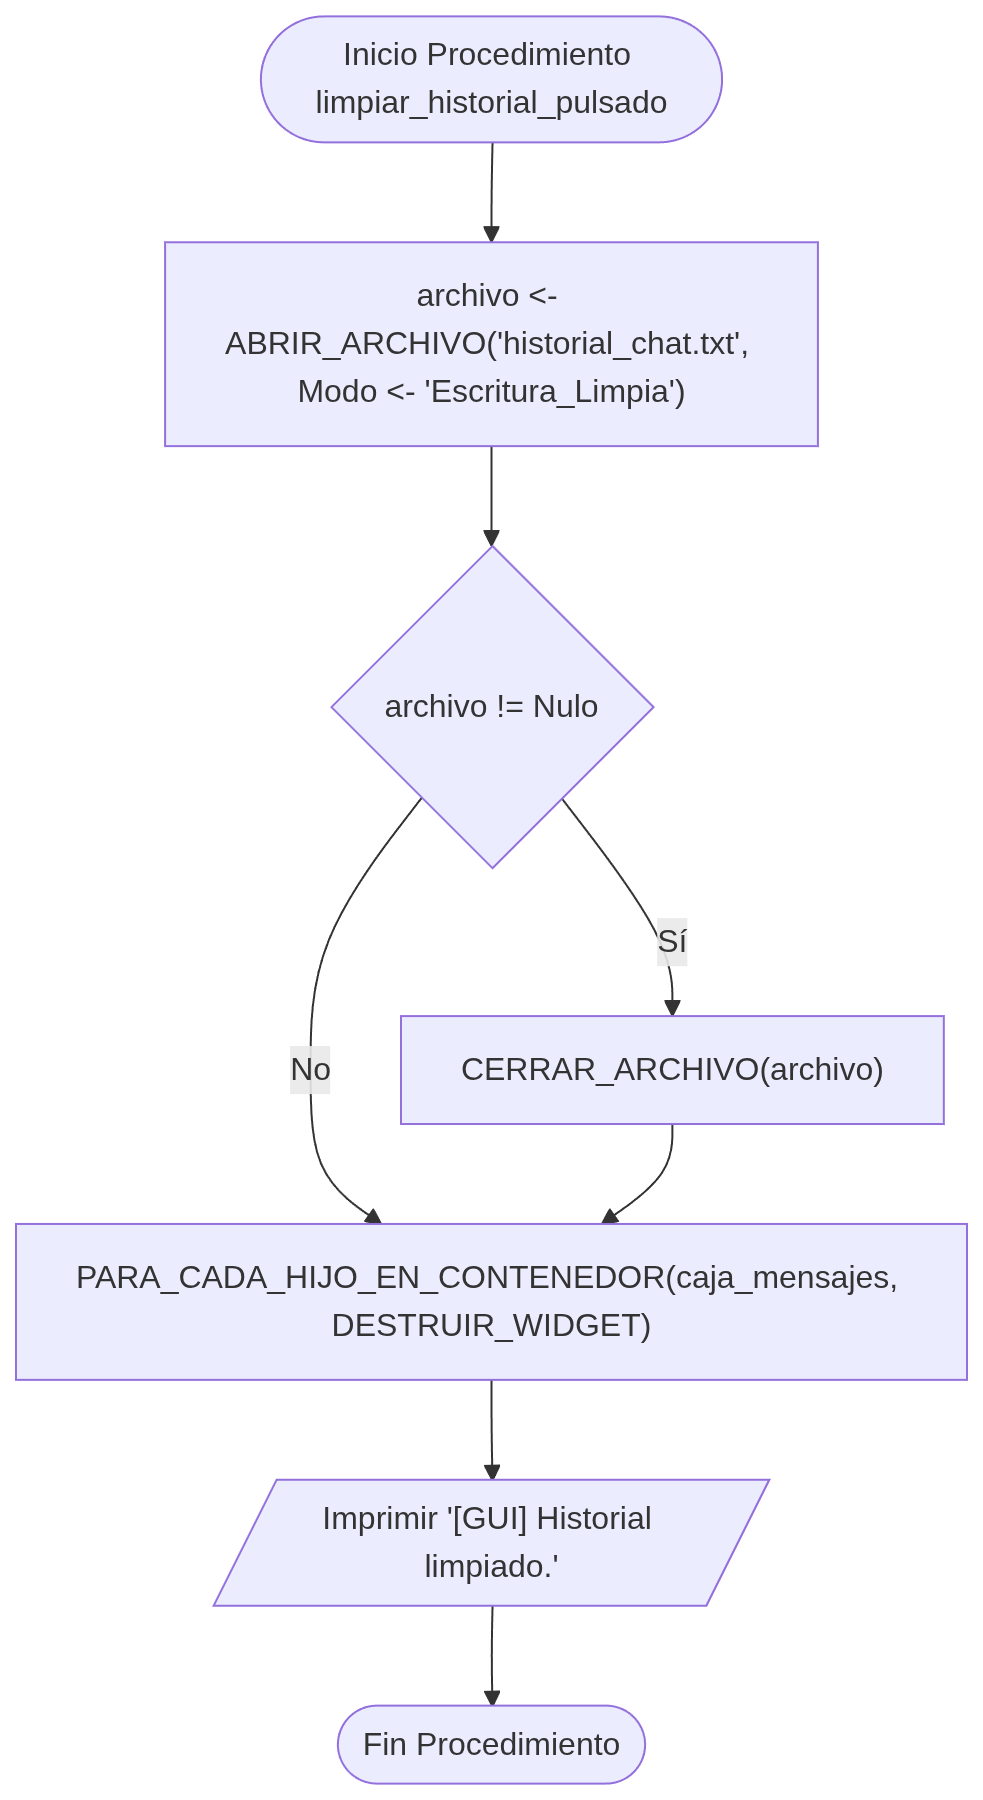
\includegraphics[width=0.4\textwidth]{Diagramas3/limpiar_historial_pulsado.png} 
\end{figure}

% --- FUNCION 10 ---
\newpage
\paragraph{10. Función \texttt{scroll\_al\_final()}} ~\\
\begin{figure}[H]
    \centering
    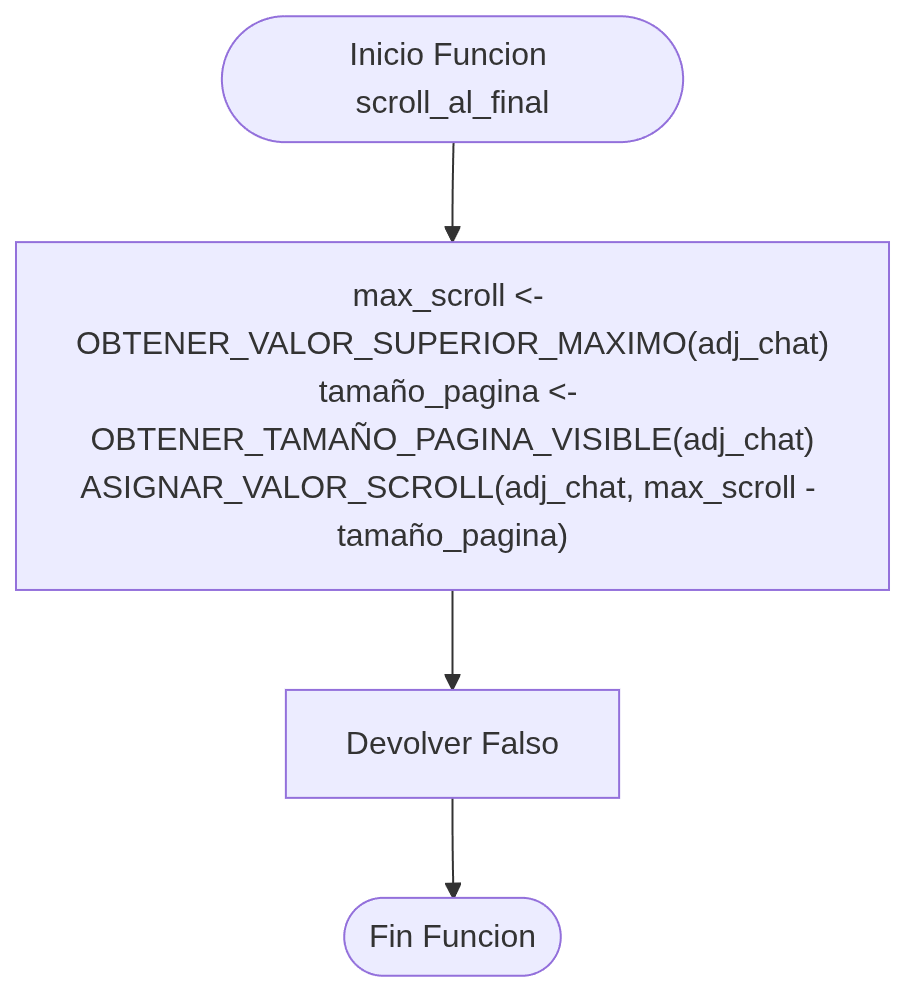
\includegraphics[width=0.4\textwidth]{Diagramas3/scroll_al_final.png} 
\end{figure}

% --- FUNCION 11 ---
\paragraph{11. Función \texttt{mostrar\_mensaje\_recibido()}} ~\\
\begin{figure}[H]
    \centering
    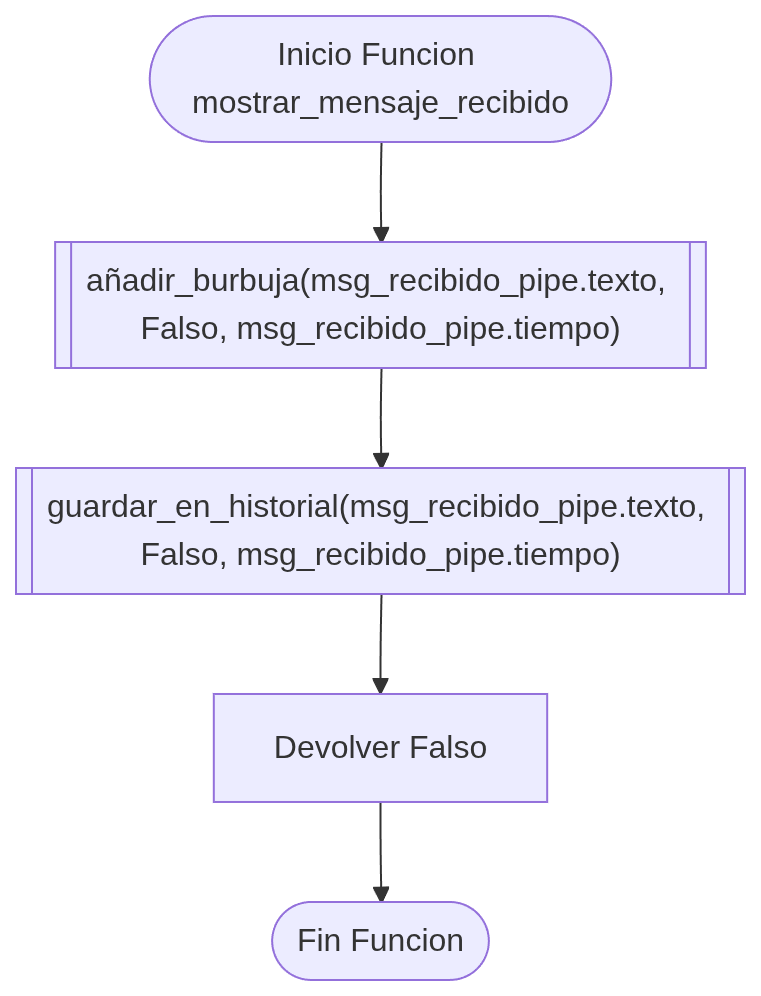
\includegraphics[width=0.4\textwidth]{Diagramas3/mostrar_mensaje_recibido.png} 
\end{figure}

% --- PROCEDIMIENTO 12 ---
\newpage
\paragraph{12. Procedimiento \texttt{cargar\_css()}} ~\\
\begin{figure}[H]
    \centering
    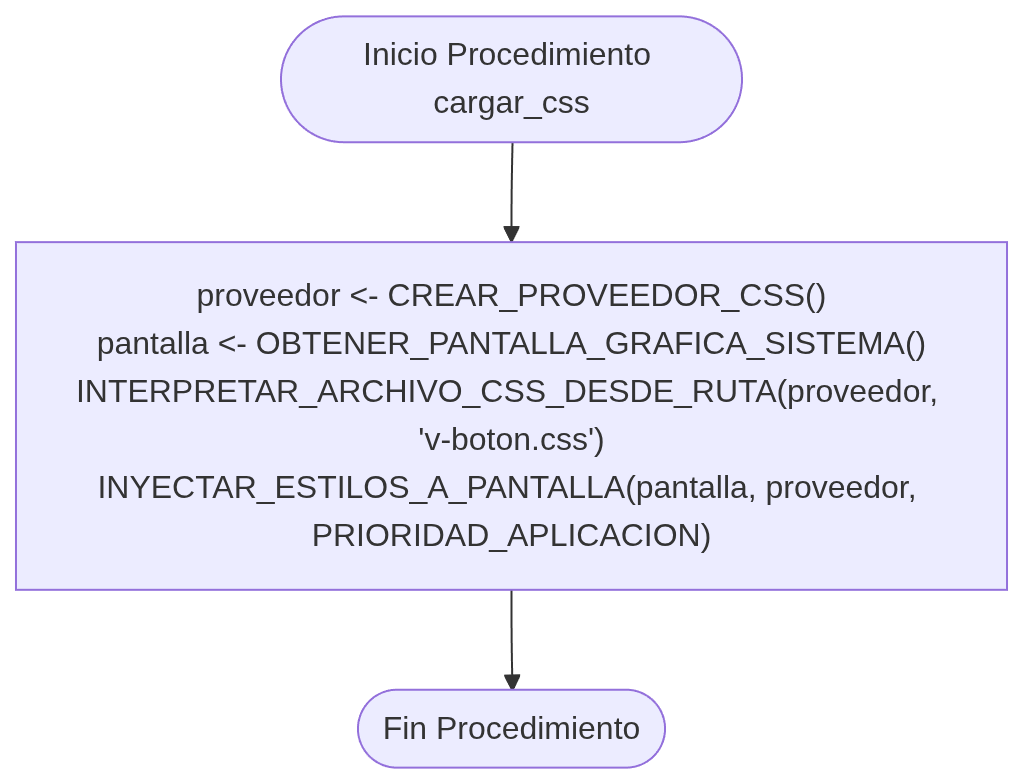
\includegraphics[width=0.4\textwidth]{Diagramas3/cargar_css.png} 
\end{figure}